\begin{figure}[h]
    \centering
    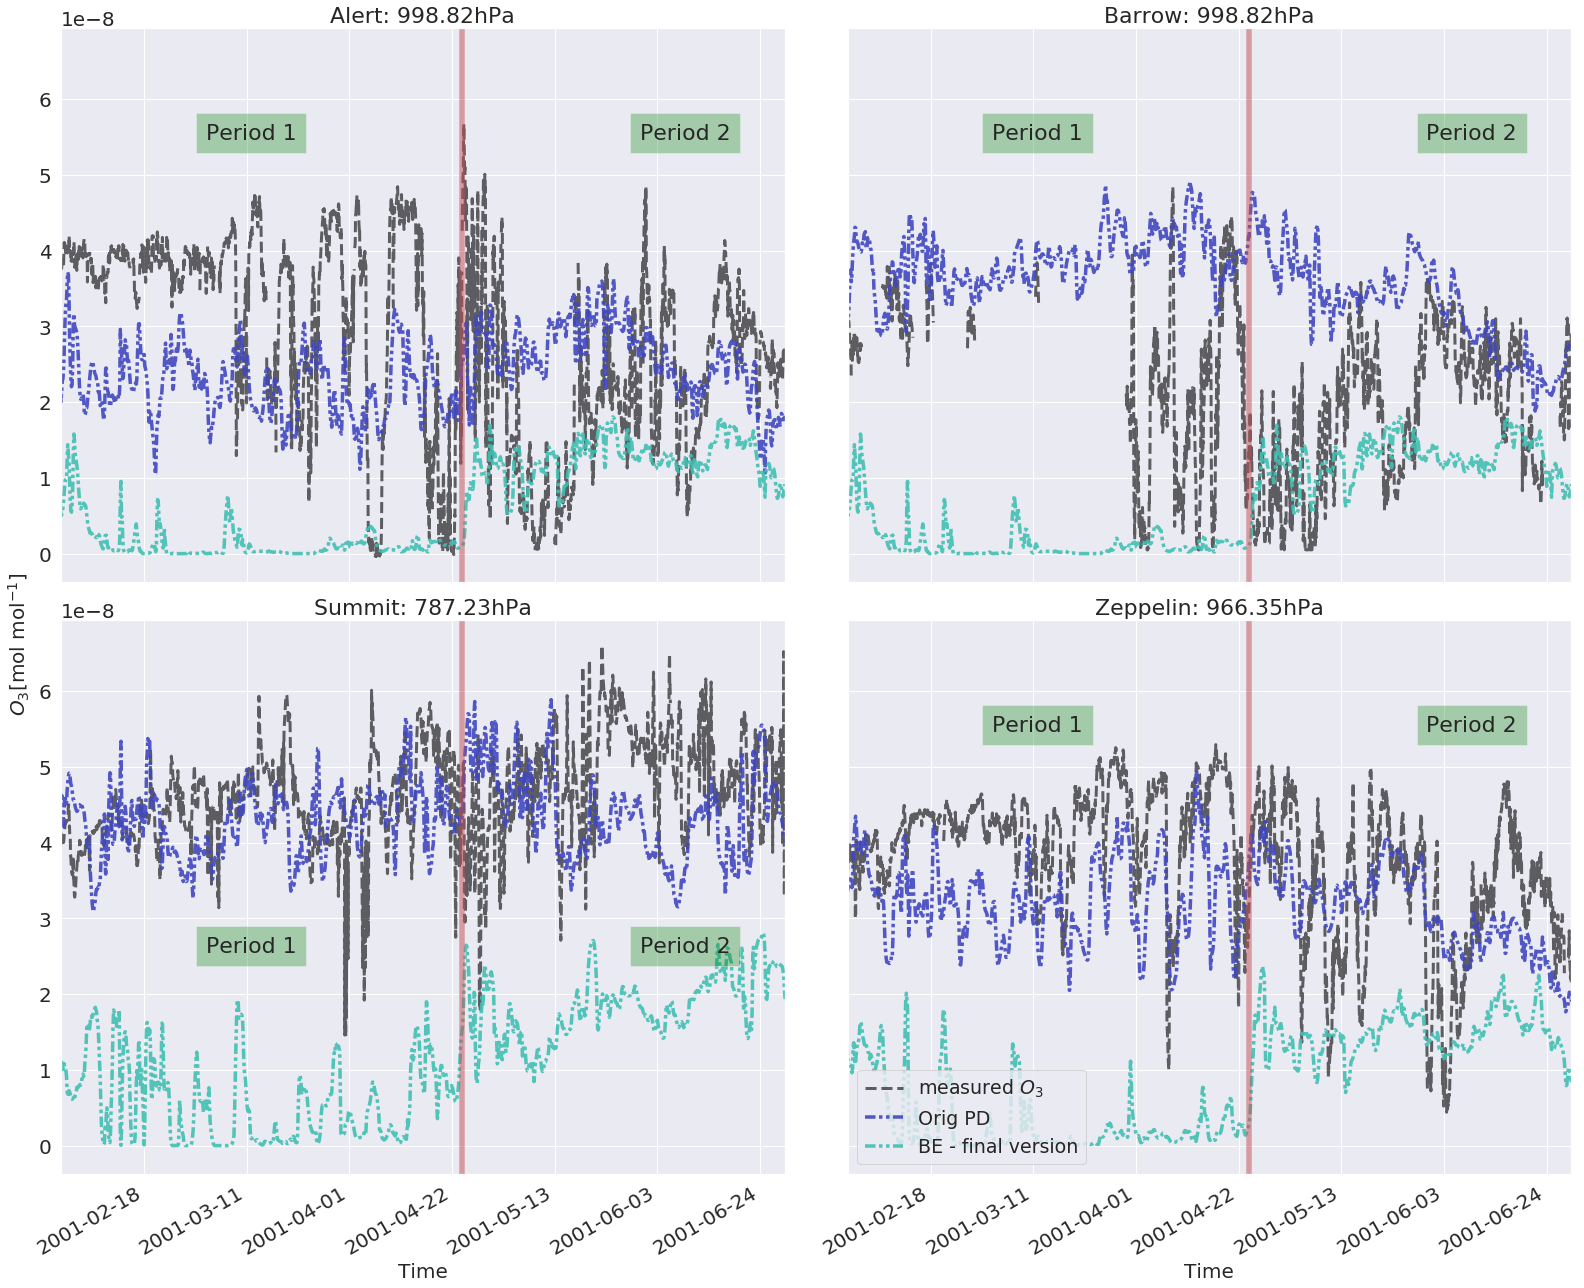
\includegraphics[width = \linewidth]{Chapter6_Results/images/ozone_stationComp_2001/ozone_2001_2periods_step5.png}
    \caption{Ozone measurements (black line) and model results from the original CTM3 (Branch \ref{def:origCTM3_PD}) (blue line) and the final version of the halogen branch (turquoise line) at the four different stations, Alert (top left), Barrow (top right), Summit (lower left) and Zeppelin (lower right) with measurements and model results from February to June, 2001. The results are split into two periods, 'Period 1' and 'Period 2' and the vertical line represents the separation between the periods. Model results were taken from the approximate altitude of the station in hPa}
    \label{fig:2p_step5}
\end{figure}